% Activate the following line by filling in the right side. If for example the name of the root file is Main.tex, write
% "...root = Main.tex" if the chapter file is in the same directory, and "...root = ../Main.tex" if the chapter is in a subdirectory.
 
%!TEX root =  

\chapter[Systematic Errors]{Systematic Errors}

\section{Systematic Errors on the Signal}
\subsection{Trigger Efficiency}
\label{sec:trigger_syst}
\subsection{Jet Energy Scale and Resolution}
\subsection{Signal Monte Carlo Generator Systematics}

\section{Systematic Errors on the Background Estimation}
\subsection{Systematic Errors on Data-Driven Background Estimates}
Validating the matrix method predictions of the $m_{bb}$ shap is a bit more subtle. 
Since we use the matrix method to help validate our assumption that mbb of the leading 2 jets is independent of the truth
 flavor of the third jet, we need to demonstrate that the matrix method reweighting does not distort the
 mbb shape. We test this by generating toy MC distributions where our assumption is incorrect (by design,
 we make the mbb distribution dependent on the truth flavor of the 3rd jet) and then run those toy events
 through the matrix method to check if the different distributions are projected out correctly.
 Using the $m_{bb}$ distribution in data as a template, we generate three $m_{bb}$ distributions that have different
 shapes (the $m_{bb}$ values are scaled down by 7\% for light jets, left unchanged for charm jets, and scaled
 up by 15\% for bottom jets), and draw an $m_{bb}$ value at random from one of those distributions depending
 on the truth flavor. These different $m_{bb}$ distributions are not meant to model the data in any physically
 relevant way, but rather to guarantee that if there are systematic differences in $m_{bb}$ that are correlated
 with the flavor of the third jet, the matrix method will get the $m_{bb}$ shape correct.
 The results of this study can be seen in Figure~\ref{fig:mbb_compare_truth_mm_toy}; it is clear that the 
shape differences in the original distributions propagate through to the matrix method predictions.



\begin{figure}
    \centering
    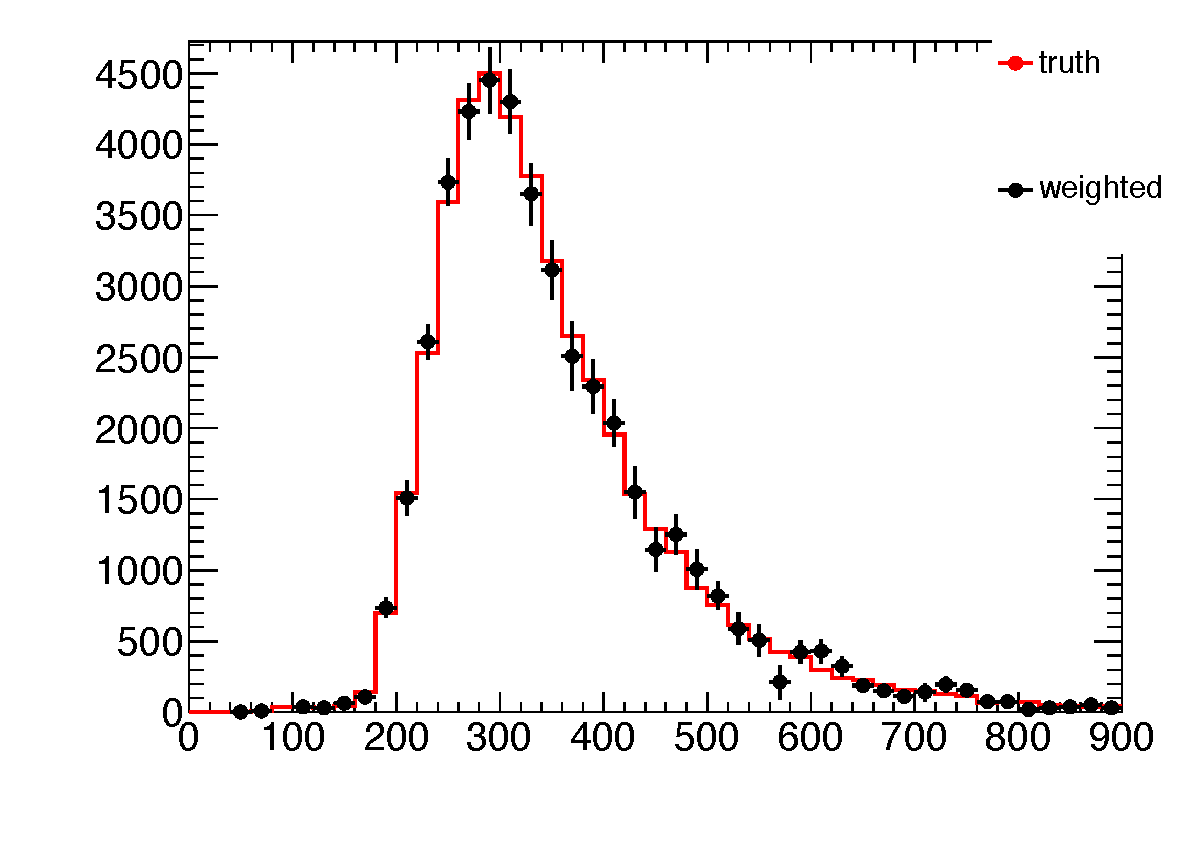
\includegraphics[width=0.3\linewidth]{Systematics/mm_shape_check_b.pdf}
    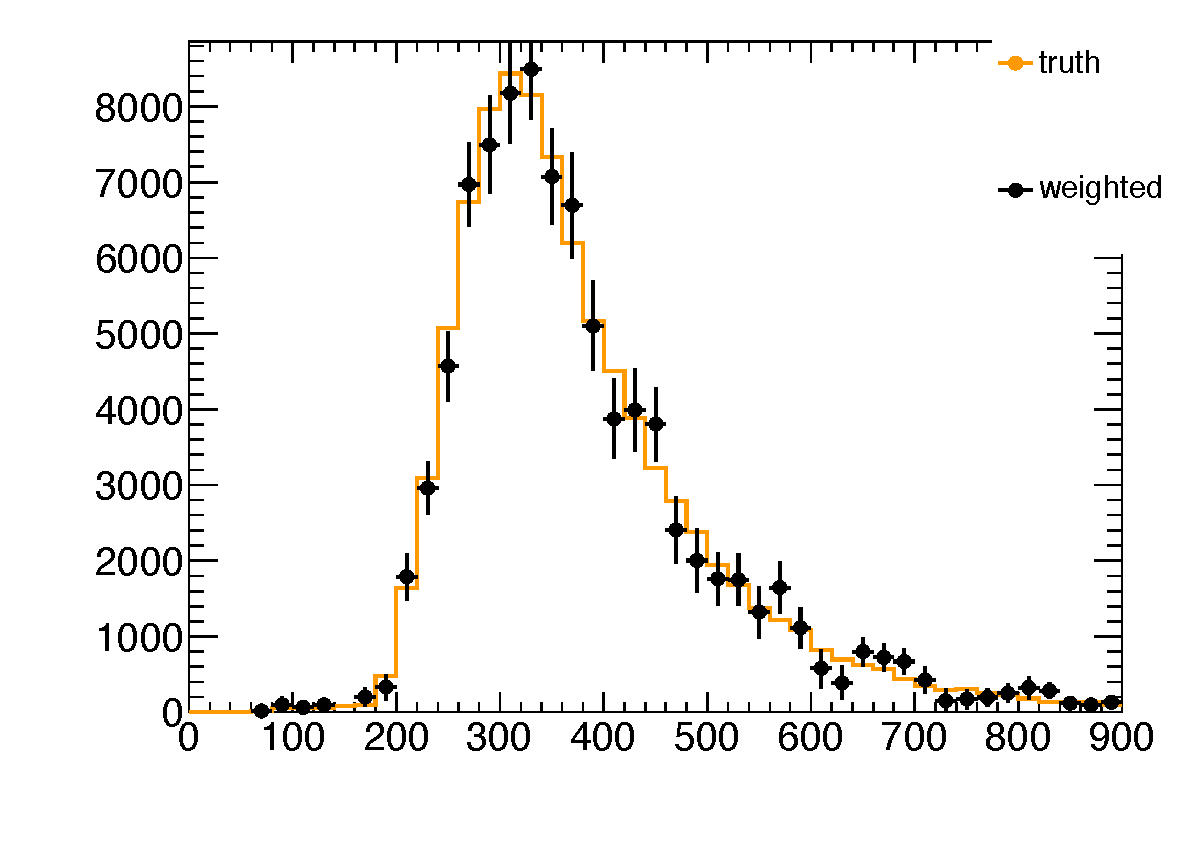
\includegraphics[width=0.3\linewidth]{Systematics/mm_shape_check_c.pdf}
    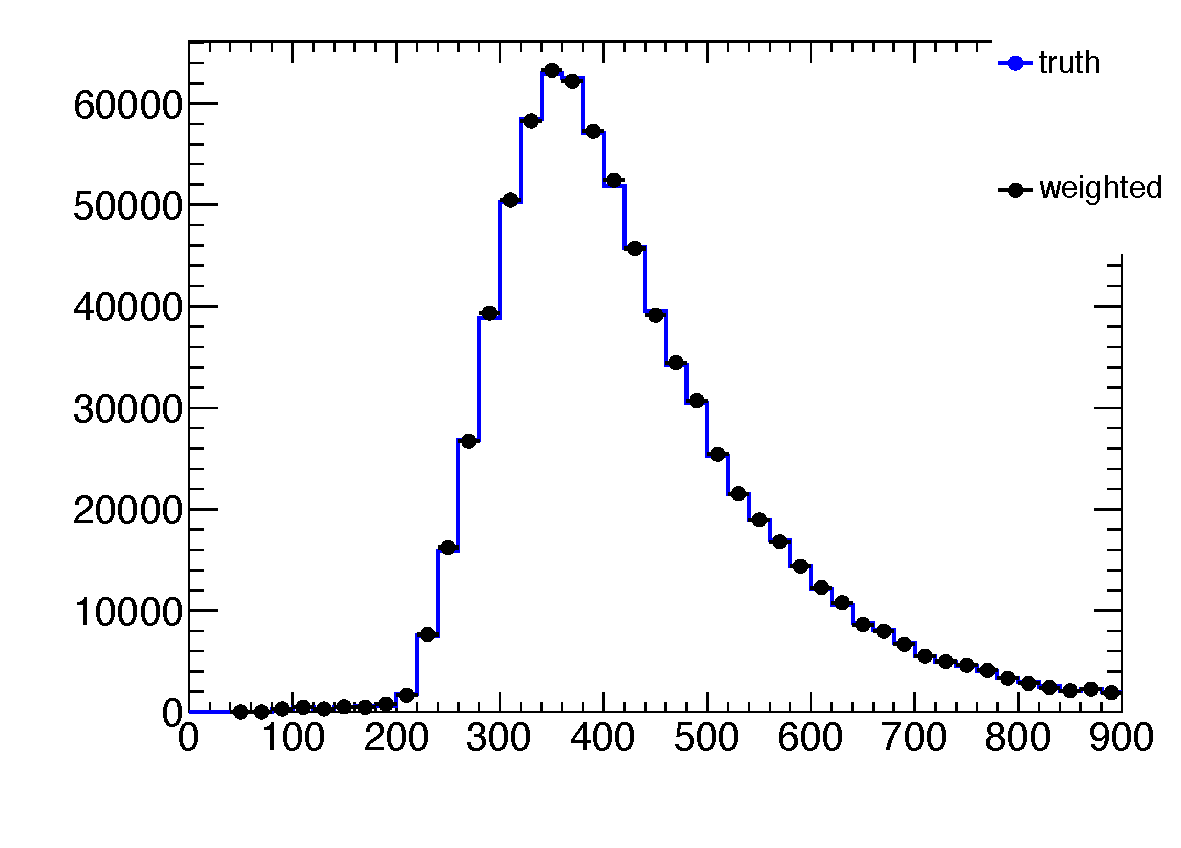
\includegraphics[width=0.3\linewidth]{Systematics/mm_shape_check_light.pdf}
    \caption{A comparison of the toy $m_{bb}$ distributions for the different flavors of the
        third jet, as shown in Figure~\ref{fig:mbb_compare_truth_spectra}, with the matrix
        method predictions overlaid.  }
    \label{fig:mbb_compare_truth_mm_toy}
\end{figure}


\subsubsection{$b$-Tagging Scale Factors}
\label{sec:SF}
Although every effort is made to accurately simulate the production rates and
kinematic properties of $b$-quarks, as well as the performance of the ATLAS
detector, it is difficult to imagine that Monte Carlo simulation perfectly represents
the b-tagging efficiencies that might be found in data.  At the same time, it
is challenging to derive pure data-driven samples of $b$, $c$ and light jets to which
the b-tagging can then be applied, and used to derive the efficiencies:

    \begin{equation}
        eff_{b,c,light}=\frac{number\ of\ truth\ b,\ c,\ light}{number\ of\ tagged\ b,\ c,\ light}
    \end{equation}

Scale factors are computed by the flavor tagging performance group to quantify the
difference between the data and MC efficiencies.

    \begin{equation}
        eff_{data}=eff_{MC}\times SF_{data}
    \end{equation}


The eigenvector method is used to derive a set of independent variations of the data-MC scale
factors, in such a way to take the full covariance matrix of the calibration measurements
into account, including correlations among working points and different jet $p_{T}$ regions.
For further explanation of the eigenvector method please see section 2.3 of% ~\ref{ref:VHBTagging}. 
%GP Soon we can reference the cont. tagging conf note (for now ATLAS-COM-CONF-2014-003).

The scale factors used in this analysis are grouped by whether they are applied to jets in the
tight, loose or anti-tagged bins.  The nominal values for the scale factors, as well as the results
given by the eigenvector variations, and can be found in Appendix~\ref{sec:SF}.

When the eigenvector variations are applied and their effect propagated through the matrix method,
we can ask what the effect is on the total number of $b$, $c$, and light jets predicted.
There are 12 variations each for $b$ and $c$ jets, and 24 variations for light jets, so
overall there are 48 variations that need to be examined.

\begin{figure}[hbt]
  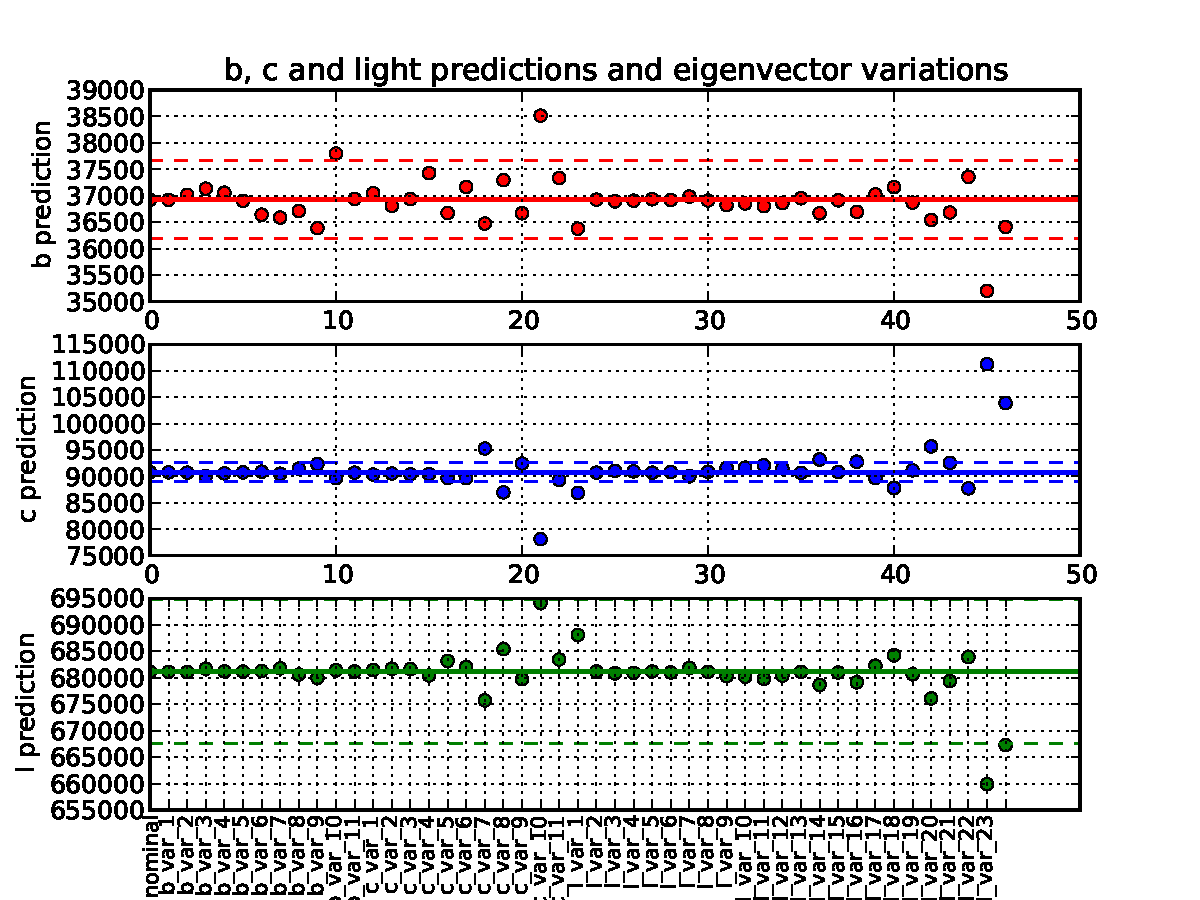
\includegraphics[width=0.98\linewidth]{Systematics/eigenvector_variations.pdf}
  \caption{The changes in flavor predictions in data due to eigenvector variations.  Th
    colored line in each subplot shows the nominal prediction given by the matrix method;
    each point is the prediction generated when a different eigenvector variation is applied.
    The variations are labeled on the x axis.  The colored dotted lines show the +\- 2\%
    envelope for the nominal prediction.}
  \label{fig:eigenvector_variations}
\end{figure}

\subsection{Systematic Errors on MC-Derived Background Estimates}





